%\setcounter{chapter}{0}
\renewcommand{\theequation}{\thechapter.\arabic{equation}}
\numberwithin{equation}{chapter}

\chapter{กฎการเคลื่อนที่ของนิวตัน}
\label{Chapter:NewtonLaw}
\renewcommand{\thesection}{\thechapter.\arabic{section}}
\renewcommand{\theequation}{\thesection.\arabic{equation}}
\numberwithin{equation}{section}


%\section*{จุดประสงค์}
%\addtocontents{toc}{จุดประสงค์}


%--------------------------------------------------------------------------------------

% \section{กลศาสตร์คลาสสิก}
% \label{Sec:ClassicalMechanics}

% วิชากลศาสตร์ (Mechanics) เป็นการศึกษาว่าสิ่งต่างๆมีการเคลื่อนที่ได้อย่างไร เช่น ดาวเคราะห์โคจรรอบดวงอาทิตย์ได้อย่างไร, นักสกีเคลื่อนที่ลงทางลาดชันได้อย่างไร, หรืออิเล็กตรอนเคลื่อนที่รอบนิวเคลียสในอะตอมได้อย่างไร เป็นต้น นานมาแล้วเราทราบว่าชาวกรีกเป็นชนกลุ่มแรกที่คิดเกี่ยวกับวิชากลศาสตร์อย่างจริงจังมามากกว่า
% สองพันปีก่อน วิชากลศาสตร์ของชาวกรีกได้แสดงให้เห็นขั้นตอนของการวิวัฒนาการของวิทยาศาสตร์สมัยใหม่
% อย่างเป็นขั้นตอน แต่อย่างไรก็ตาม แนวคิดของชาวกรีกในยุคนั้นก็ยังมีข้อผิดพลาดที่ร้ายแรงตามมาตรฐานของยคสมัยใหม่ แต่เราก็จะไม่สนใจในเอกสารนี้ การพัฒนาของวิชากลศาสตร์ที่เรารู้จักกันในปัจจุบันเริ่มต้นจากงานของกาลิเลโอ (Galileo) (ค.ศ. 1564 - ค.ศ. 1642) และนิวตัน (Newton) (ค.ศ. 1642 - ค.ศ. 1727) และจากการคิดกฎการเคลื่อนที่สามข้อของนิวตัน ซึ่งนั่นจะเป็นจุดเริ่มต้นเของเราในเอกสารนี้

% ในช่วงปลายของศตวรรษที่ 18 และตอนต้นของศตวรรษที่ 19 การพัฒนาวิชากลศาสตร์ได้มีสองแนวทางที่แตกต่างจากวิชากลศาสตร์ของนิวตัน ซึ่งได้เรียกตามชื่อของผู้คิดค้น ได้แก่ นักคณิตศาสตร์และดาราศาสตร์ชาวฝรั่งเศส ``ลากรางจ์" (Lagrange) (ค.ศ. 1736 - ค.ศ. 1813) เรียกว่า ``กลศาสตร์ลากรางจ์" และนักคณิตศาสตร์ชาวไอริส ``ฮามิลตัน" (Hamilton) (ค.ศ. 1805 - ค.ศ. 1865) เรียกว่า ``กลศาสตร์ฮามิลตัน" สำหรับแนวทางของกลศาสตร์ลากรางจ์ และกลศาสตร์ฮามิลตันนั้นมีความสอดคล้องกับกลศาสตร์นิวตัน
%  แต่แนวทางทั้งสองนี้สามารถจัดการแก้ปัญหาต่างๆที่มีความสลับซับซ้อนได้ดีกว่ากลศาสตร์นิวตัน และยังมีการเลียนแบบในหลากหลายด้านในการพัฒนาแนวคิดยุคใหม่ ในบริบทของคำว่า ``กลศาสตร์คลาสสิก" (Classical Mechanics) นั้นบางครั้งก็ยังคงไม่ชัดเจน แต่ตามความเข้าใจโดยทั่วไป ก็จะหมายความถึงกลศาสตร์ทั้งสามแนวทางนี้

% จนกระทั่งในช่วงเริ่มต้นของศตวรรษที่ยี่สิบ ดูเหมือนว่า กลศาสตร์คลาสสิก จะกลายเป็น\textit{ส่วนหนึ่ง}ในวิชากลศาสตร์เท่านั้น พูดให้ถูกต้องคือ เฉพาะส่วนที่อธิบายถึงการเคลื่อนที่ทุกชนิดที่เป็นไปได้นั่นเอง ในภายหลัง ในช่วงยี่สิบปีนับตั้งแต่ปี ค.ศ. 1905 ถึง ค.ศ. 1925 เป็นที่ทราบกันอย่างชัดเจนว่ากลศาสตร์คลาสสิกไม่สามารถอธิบายการเคลื่อนที่ของวัตถุที่มีการเคลื่อนที่
% ด้วยอัตราเร็วใกล้อัตราเร็วของแสงได้อย่างถูกต้อง และยังไม่สามารถอธิบายถึงอนุภาคขนาดเล็ก (microscopic particles) ภายในอะตอมและโมเลกุลได้อย่างถูกต้องเช่นกัน ผลของมันทำให้เกิดการพัฒนากลศาสตร์รูปแบบใหม่สองแนวทางที่สมบูรณ์แบบขึ้นมา นั่นคือ กลศาสตร์สัมพัทธภาพ (Relativistic Mechanics) สำหรับใช้อธิบายการเคลื่อนที่ด้วยอัตราเร็วสูง และกลศาสตร์ควอนตัม (Quantum Mechanics) สำหรับใช้อธิบายการเคลื่อนที่ของอนุภาคขนาดเล็ก 

% แม้ว่ากลศาสตร์คลาสสิกจะถูกแทนที่ด้วยกลศาสตร์สัมพัทธภาพ และกลศาสตร์ควอนตัมในแต่ละแนวทาง แต่ยังมีช่วงของความสนใจ และปัญหาที่น่าสนใจที่กว้างขวาง ซึ่งกลศาสตร์คลาสสิกสามารถใช้อธิบายได้อย่างสมบูรณ์และถูกต้องในเรื่องการเคลื่อนที่เหล่านั้น โดยเฉพาะอย่างยิ่งกับการมาถึงของทฤษฎีความยุ่งเหยิง (Chaos Theory) ในช่วงสิบยี่สิบปีล่าสุดนี้ การศึกษาวิจัยด้านกลศาสตร์คลาสสิกมีความเข้มข้นมากขึ้นและหัวข้อเหล่านั้นก็ได้รับความสนใจอย่าง
% มากในวงการฟิสิกส์

% \section{อวกาศและเวลา}
% \label{Sec:SpaceAndTime}

% กฎการเคลื่อนที่สามข้อของนิวตัวได้มีแนวคิดพื้นฐานที่สำคัญอยู่สี่อย่าง คือ แนวคิดเกี่ยวกับอวกาศ (space), เวลา (time), มวล (mass) และแรง (force) ในหัวข้อนี้เราจะทำการพูดถึงสองสิ่งแรกก่อน นั่นคือ อวกาศกับเวลา โดยจะอธิบายถึงมุมมองแบบคลาสสิกเกี่ยวกับอวกาศและเวลา ซึ่งจะทบทวนเรื่องของเวกเตอร์เล็กน้อยก่อนที่จะพูดถึงการระบุจุดในอวกาศ

% \subsection{อวกาศ}
% \label{SubSec:Space}

% แต่ละจุด $P$ ในอวกาศสามมิติที่เราอาศัยอยู่นี้ สามารถระบุได้โดยเวกเตอร์ตำแหน่ง $\vec{r}$ ซึ่งสามารถระบุขนาดและทิศทางของจุด $P$ จากจุดกำเนิด $O$ ดังรูปที่ \ref{Fig2.1} การระบุเวกเตอร์นี้สามารถทำได้หลายวิธี แต่วิธีหนึ่งที่คุ้นเคยกันดีคือการบอกในรูปของพิกัด ($x$, $y$, $z$) ในระบบพิกัดฉาก วิธีการที่นิยมก็มักจะระบุค่าพร้อมกับเวกเตอร์หน่วย (unit vector) คือ $\x$, $\y$, $\z$ ที่มีทิศทางชี้ไปตามแนวแกนทั้งสามของระบบพิกัดฉาก และเราสามารถเขียนเวกเตอร์ตำแหน่งได้ดังนี้
% \begin{equation}\label{Eqn:PosVecR}
% \vec{r} = x\x + y\y + z\z
% \end{equation}

% ในงานพื้นฐาน มันจะดีกว่าถ้าเราเลือกใช้สัญลักษณ์อย่างที่ใช้ในสมการที่ (\ref{Eqn:PosVecR}) และใช้มันไปเรื่อยๆ สำหรับในงานที่มีระดับที่ยากขึ้นไป มันแทบจะเป็นไปไม่ได้เลยที่จะหลีกเลี่ยงการใช้สัญลักษณ์ที่แตกต่างกันมากมาย ผู้แต่งตำราต่างกันก็มักจะมีการใช้สัญลักษณ์ที่แตกต่างกันไปด้วย (ตัวอย่างสัญลักษณ์ของเวกเตอร์หน่วยที่นิยมกันแบบอื่น คือ การใช้ในรูปแบบ $\i$, $\j$, $\k$ แต่ในเอกสารนี้จะใช้รูปแบบ\footnote{ในที่นี้ผู้แปลจะใช้สัญลักษณ์ $\x$, $\y$, $\z$ แทนเวกเตอร์หน่วย เช่นเดียวกันกับตำราต้นฉบับ สำหรับเนื้อหานับจากนี้เป็นต้นไป ซึ่งอาจจะแตกต่างจากเนื้อหาในบทแรก ที่มีการใช้สัญลักษณ์แทนเวกเตอร์หน่วยด้วย $\i$, $\j$, $\k$} $\x$, $\y$, $\z$ ยิ่งกว่านั้น สัญลักษณ์แทบทุกแบบมักมีข้อบกพร่องของมันเอง ซึ่งสามารถทำให้มีความไม่เหมาะสมในการใช้งานในบางโอกาส 

% \begin{figure}%[!h]%%Figure 2.1
% \centering
% 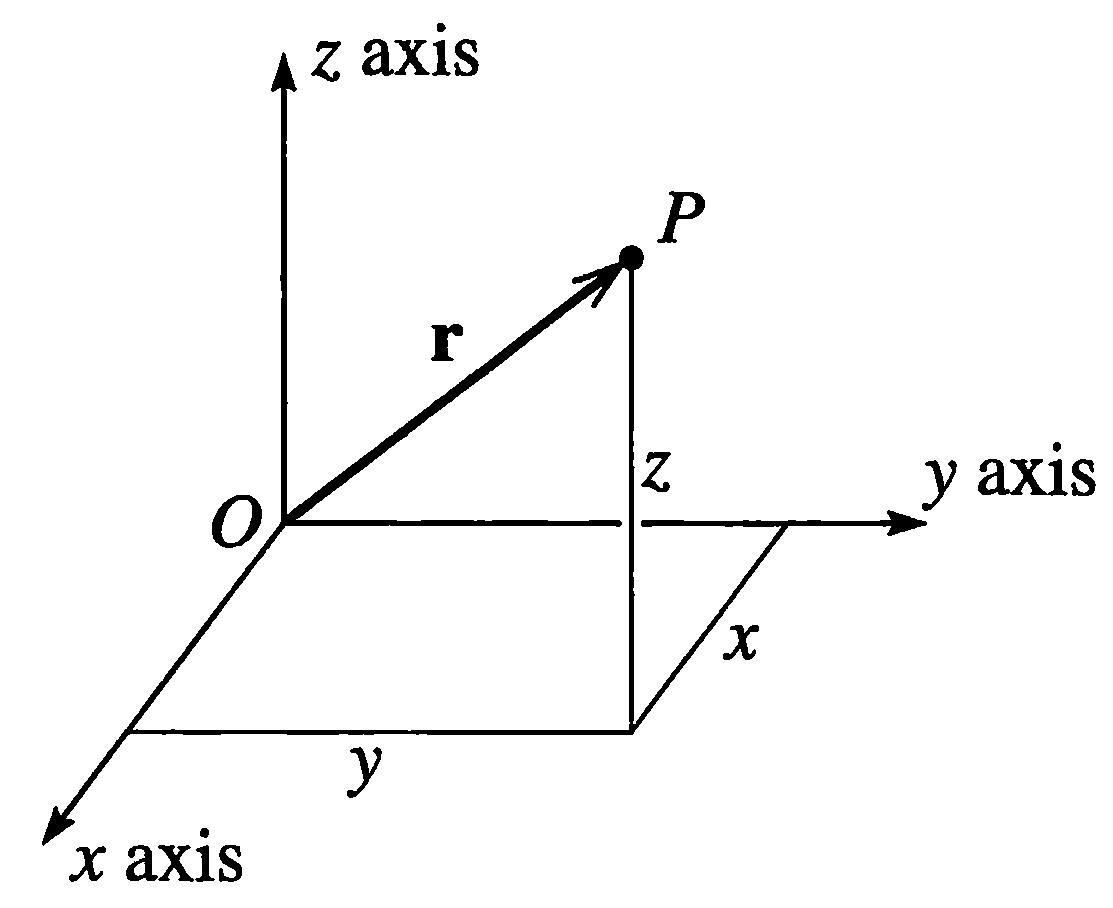
\includegraphics[width=0.5\columnwidth]{Fig2.1.png}
% \caption{จุด $P$ ถูกระบุด้วยเวกเตอร์ตำแหน่ง $\vec{r}$ ซึ่งบอกถึงระยะของจุด $P$ เทียบกับจุดกำเนิด $O$ โดยเวกเตอร์ตำแหน่ง $\vec{r}$ สามารถระบุได้ด้วยพิกัด ($x$, $y$, $z$) สัมพันธ์กับแกน $Oxyz$}
% \label{Fig2.1}
% \end{figure}

% บางครั้ง จะเป็นการสะดวกกว่า ถ้าเราจะเขียนการบอกเวกเตอร์ตำแหน่งแบบย่อๆ จากสมการที่ (\ref{Eqn:PosVecR}) สามารถเขียนย่อได้เป็น
% \begin{equation}\label{Eqn:PosVecRShort}
% \vec{r} = (x, y, z)
% \end{equation}
% จะเห็นว่าสัญลักษณ์นี้ไม่สอดคล้องกับสมการที่ (\ref{Eqn:PosVecR}) เท่าไรนัก แต่มันก็สมบูรณ์แบบชัดเจน และยืนยันได้ว่า $\vec{r}$ เป็นปริมาณเวกเตอร์ที่มีองค์ประกอบเป็น $x$, $y$, $z$ จริงๆ เมื่อสัญลักษณ์ดังสมการที่ (\ref{Eqn:PosVecRShort}) มีความสะดวกมากกว่า เราก็จะใช้ในรูปแบบนี้เป็นหลัก สำหรับปริมาณเวกเตอร์ทั้งหลาย เราจะระบุองค์ประกอบแต่ละแนวแกนด้วยตัวห้อย $x$, $y$, $z$ เช่น เวกเตอร์ความเร็ว $\vec{v}$ จะมีองค์ประกอบแต่ละแนวแกนเป็น $v_x$, $v_y$, $v_z$, เวกเตอร์ความเร่ง $\vec{a}$ จะมีองค์ประกอบแต่ละแนวแกนเป็น $a_x$, $a_y$, $a_z$ เป็นต้น

% เมื่อสมการของเรามีความซับซ้อนมากขึ้น มันคงไม่สะดวกถ้าเราจะเขียนองค์ประกอบขอ
% สมการทั้งสามในรูปการบวกกันแบบสมการที่ (\ref{Eqn:PosVecR}) ดังนั้นส่วนใหญ่มักใช้เครื่องหมายสัญลักษณ์การบวก $\sum$ แทนเพื่อให้สามารถเขียนได้ในพจน์เดียว ในการนี้บางครั้งสำหรับองค์ประกอบทั้งสามในแนวแกน $x$, $y$, $z$ ของเวกเตอร์ตำแหน่ง $\vec{r}$ จะถูกเขียนใหม่ในรูป $r_1$, $r_2$, $r_3$ และเวกเตอร์หน่วยทั้งสาม $\x$, $\y$, $\z$ ก็จะถูกเขียนใหม่เป็น $\e{1}$, $\e{2}$, $\e{3}$ ด้วยเช่นกัน นั่นคือ เราจะนิยามองค์ประกอบ
% \begin{equation}\label{Def:Rcomp}
% r_1 = x, \hspace{1cm} r_2 = y, \hspace{1cm} r_3 = z,
% \end{equation}
% และเวกเตอร์หน่วย
% \begin{equation}\label{Def:UnitVecE}
% \e{1} = \x, \hspace{1cm} \e{2} = \y, \hspace{1cm} \e{3} = \z
% \end{equation}
% เมื่อสัญลักษณ์ $\hat{e}$ นี้ใช้แทนเวกเตอร์หน่วย ($e$ นี้มาจากภาษาเยอรมันจากคำว่า ``eins" ซึ่งแหละว่า ``หนึ่ง") และจากการใช้สัญลักษณ์แบบนี้ สมการที่ (\ref{Eqn:PosVecR}) จะสามารถเขียนได้เป็น
% \begin{equation}\label{Eqn:PosVecRinE}
% \vec{r} = r_1\e{1} + r_2\e{2} + r_3\e{3} = \sum_{i=1}^{3}r_i\e{i}
% \end{equation}
% จากสมการที่มีรูปแบบง่ายๆ ดังสมการที่ (\ref{Eqn:PosVecRinE}) นั้นไม่ได้มีประโยชน์มากกว่าสมการที่ (\ref{Eqn:PosVecR}) เลย เพียงแต่มีความสะดวกในการเขียนมากว่าเท่านั้นเอง

% \subsection{การดำเนินการทางเวกเตอร์}
% \label{SubSec:VectorOperations}

% ในการเรียนวิชากลศาสตร์ เราจะได้เจอการดำเนินการหลายแบบซ้ำๆที่ดำเนินการกับเวกเตอร์ ถ้า $\vec{r}$ และ $\vec{s}$ เป็นปริมาณเวกเตอร์ที่มีองค์ประกอบ เป็น $\vec{r} = (r_1, r_2, r_3)$ และ $\vec{s} = (s_1, s_2, s_3)$ แล้วการ$\textbf{บวก}$ (หรือการหาผลลัพธ์) ของ $\vec{r} + \vec{s}$ จะหาได้จากการบวกขององค์ประกอบแต่ละแนวแกน นั่นคือ
% \begin{equation}\label{Eqn:VectorSum}
% \vec{r} + \vec{s} = (r_1 + s_1, r_2 + s_2, r_3 + s_3)
% \end{equation}
% ตัวอย่างทำสำคัญของการบวกเวกเตอร์ คือ การหาแรงลัพธ์ที่กระทำต่อวัตถุ คือ เมื่อมีแรงสองแรง $\vec{F}_a$ และ $\vec{F}_b$ กระทำต่อวัตถุชิ้นหนึ่ง ผลที่ได้จะเหมือนกับมีแรงหนึ่งแรง ที่เรียกว่าแรงลัพธ์ (resultant force) ที่เกิดจากการบวกเวกเตอร์แรง
% \begin{equation}\label{Eqn:VecSum2F}
% \vec{F} = \vec{F}_a + \vec{F}_b
% \end{equation}
% ซึ่งจะเหมือนเช่นเดียวกันกับกฎการบวกเวกเตอร์ สมการที่ (\ref{Eqn:VectorSum})

% ถ้า $c$ เป็นปริมาณสเกลาร์ (หรือก็คือ ตัวเลขใดๆ) และ $\vec{r}$ เป็นปริมาณเวกเตอร์ $\textit{ผลคูณ} c\vec{r}$ สามารถหาได้จาก
% \begin{equation}\label{Eqn:VectorProduct}
% c\vec{r} = (cr_1, cr_2, cr_3)
% \end{equation}
% นั่นหมายความว่า $c\vec{r}$ เป็นปริมาณเวกเตอร์ที่มีทิศทางเดียวกัน\footnote{ทั้งนี้ถ้าค่าของสเกลาร์ $c$ มีค่าเป็นลบ ผลคูณ $c\vec{r}$ จะมีทิศทาง$\textit{ตรงกันข้ามกัน}$กับเวกเตอร์ $\vec{r}$}กับเวกเตอร์ $\vec{r}$ และมีขนาดเท่ากับค่าของ $c$ คูณกับขนาดของเวกเตอร์ $\vec{r}$ ตัวอย่างที่สำคัญอันหนึ่งคือตามกฎการเคลื่อนที่ข้อที่สองของนิวตัน แรงลัพธ์ $\vec{F}$ ที่กระทำกับวัตถุจะมีค่าเท่ากับผลคูณ $m\vec{a}$ เสมอ ดังสมการที่ (\ref{Eqn:VectorProduct})

% การหาผลคูณแบ่งออกเป็นสองวิธีการที่สำคัญ ซึ่งสามารถสร้างได้จากสองเวกเตอร์ใดๆ คือ $\textbf{การคูณแบบสเกลาร์ หรือ การคูณแบบดอท (scalar product or dot product)}$\footnote{สามารถดูรายละเอียดได้จากบทที่ 1 ในหัวข้อ 1.1.1 การคูณแบบดอท} ซึ่งถ้าเรามีเวกเตอร์ $\vec{r}$ กับเวกเตอร์ $\vec{s}$ เราจะหาผลคูณจากการคูณแบบนี้ได้เป็น
% \begin{eqnarray}\label{Eqn:DotProduct}
% \vec{r}\cdot\vec{s} &=& rs \cos{\theta} \no \\
% 		&=& r_1s_1 + r_2s_2 + r_3s_3 \no \\
% 		&=& \sum_{n = 1}^{3} r_ns_n
% \end{eqnarray}
% เมื่อ $r$ กับ $s$ เป็นขนาดของเวกเตอร์ $\vec{r}$ และเวกเตอร์ $\vec{s}$, $\theta$ เป็นมุมระหว่างเวกเตอร์ทั้งสอง ตัวอย่างเช่น ถ้ามีแรง $\vec{F}$ กระทำให้วัตถุมีการกระจัดเป็นระยะทางน้อยๆ $d\vec{r}$ แล้วงานที่ทำเนื่องจากแรงนี้ก็หาได้จากการคูณแบบสเกลาร์ของ $\vec{F}\cdot d\vec{r}$ แล้วจะให้ผลลัพธ์ดังสมการที่ (\ref{Eqn:DotProduct}) นั่นเอง นอกจากนี้ การคูณแบบสเกลาร์ยังใช้เพื่อหาขนาดของเวกเตอร์ เช่น การหาขนาด (หรือความยาว) ของเวกเตอร์ $\vec{r}$ ซึ่งแทนด้วยสัญลักษณ์ $|\vec{r}|$ หรือ $r$, จากการใช้ทฤษฎีปิทาโกรัส (Pythagoras's theorem) ขนาดของเวกเตอร์ $\vec{r}$ จะให้ผลลัพธ์เป็น $\sqrt{r_1^2 + r_2^2 + r_3^2}$ และจากสมการที่ (\ref{Eqn:DotProduct}) เราสามารถเขียนได้คล้ายๆกันดังนี้
% \begin{equation}\label{Eqn:MagVecR}
% r = |\vec{r}| = \sqrt{\vec{r}\cdot\vec{r}}
% \end{equation}
% การหาผลคูณแบบสเกลาร์ของ $\vec{r}\cdot\vec{r}$ มักจะเขียนย่อเป็น $\vec{r}^2$

% การคูณแบบที่สองของสองเวกเตอร์ใดๆ $\vec{r}$ และ $\vec{s}$ คือ $\textbf{การคูณแบบเวกเตอร์ หรือ การคูณ}$ $\textbf{แบบครอส (vector product or cross product)}$\footnote{สามารถดูรายละเอียดได้จากบทที่ 1 ในหัวข้อ 1.1.2 การคูณแบบครอส} โดยผลลัพธ์ที่ได้จะเป็นเวกเตอร์ตัวใหม่ คือ $\vec{p} = \vec{r}\cross\vec{s}$ และมีองค์ประกอบแต่ละแนวแกนเป็นน
% \begin{eqnarray}\label{Eqn:CompCrossProduct}
% p_x &=& r_ys_z - r_zs_y \no \\
% p_y &=& r_zs_x - r_xs_z \\
% p_z &=& r_xs_y - r_ys_x \no
% \end{eqnarray}
% หรือสามารถเขียนในรูปของการหาดีเทอร์มิแนนท์ (determinant หรือ det) ได้ดังนี้
% \begin{equation}\label{Eqn:CrossProductDet}
% \vec{r}\cross\vec{s} = \begin{vmatrix} 
% 										\x & \y & \z \\ 
% 										r_x & r_y & r_z \\ 
% 										s_x & s_y & a_z 
% 									\end{vmatrix}
% \end{equation}
% ซึ่งเวกเตอร์ผลลัพธ์ที่ได้จะเป็นเวกเตอร์ที่ตั้งฉากกับทั้งเวกเตอร์ $\vec{r}$ และเวกเตอร์ $\vec{s}$ ดังรูปที่ \ref{fig2} ของบทที่ 1 โดยมีทิศทางเป็นไปตามกฎมือขวา (right-hand rule) และขนาดมีค่าเป็น $rs \sin{\theta}$ การคูณแบบเวกเตอร์นี้มีความสำคัญในการศึกษาเกี่ยวการเคลื่อนที่แบบหมุน ตัวอย่างเช่น เมื่อมีแรง $\vec{F}$ กระทำที่จุดหนึ่งของวัตถุ และจุดนั้นมีเวกเตอร์ตำแหน่งเป็น $\vec{r}$ จากจุดกำเนิด $O$ แล้วทำให้วัตถุนั้นมีการหมุนรอบจุด $O$ เราเรียกผลของแรงที่ทำให้เกิดการหมุนนี้ว่า ทอร์ค (torque, $\Gamma$) ซึ่งนิยามมาจากการคูณแบบครอส คือ $\vec{\Gamma} = \vec{r}\cross\vec{F}$


% \subsection{อนุพันธ์ของเวกเตอร์}
% \label{SubSec:VectorDerivatives}

% กฎทางฟิสิกส์ส่วนใหญ่เกี่ยวข้องกับปริมาณเวกเตอร์ และส่วนใหญ่ของกฎเหล่านี้เกี่ยวข้องกับ$\textit{การหาอนุพันธ์}$ (derivatives) ของเวกเตอร์ การหาอนุพันธ์ของเวกเตอร์นั้นมีหลากหลายวิธี และมีวิชาที่ว่าด้วยเรื่องเหล่านี้ทั้งหมด เราเรียกว่า วิชาแคลคูลัสของเวกเตอร์ (vector calculus) สำหรับตอนนี้ เราจะพิจารณาในส่วนของการหาอนุพันธ์ของเวกเตอร์อย่างง่ายๆเท่านั้น เช่น การหาอนุพันธ์ของเวกเตอร์ที่เป็นฟังก์ชันของเวลาเทียบกับเวลา ซึ่งในที่นี้ ได้แก่ ความเร็ว (velocity) $\vec{v}(t)$ ของอนุภาค หาได้จากการหาอนุพันธ์ของเวกเตอร์ตำแหน่งของอนุภาค $\vec{r}(t)$ นั่นคือ $\vec{v} = d\vec{r}/dt$ หรือทำนองเดียวกันกับเวกเตอร์ความเร่ง ซึ่งหาได้จากการหาอนุพันธ์ของเวกเตอร์ความเร็ว นั่นคือ $\vec{a} = d\vec{v}/dt$

% นิยามของการหาอนุพันธ์ของเวกเตอร์จะคล้ายกับของสเกลาร์ เราจะพิจารณาว่า ถ้า $x(t)$ เป็นฟังก์ชันสเกลาร์ที่ขึ้นกับเวลา $t$ แล้วเราสามารถนิยามอนุพันธ์ของฟังก์ชันสเกลาร์ได้ ดังนี้
% \begin{equation}\label{Def:DerivativeXt}
% \dd{x}{t} = \lim_{\Delta t \rightarrow 0}\f{\Delta x}{\Delta t}
% \end{equation}
% เมื่อ $\Delta x = x(t + \Delta t) - x(t)$ เป็นการเปลี่ยนแปลงของ $x$ เมื่อเวลาผ่านไปจาก $t$ เป็น $t + \Delta t$ เช่นเดียวกันกับเวกเตอร์ใดๆ $\vec{r}(t)$ ซึ่งเป็นเวกเตอร์ที่ขึ้นกับเวลา $t$ เราจะนิยามอนุพันธ์ของมัน ดังนี้
% \begin{equation}\label{Def:DerivativeRt}
% \dd{\vec{r}}{t} = \lim_{\Delta t \rightarrow 0}\f{\Delta \vec{r}}{\Delta t}
% \end{equation}
% เมื่อ
% \begin{equation}\label{Def:DeltaRfn}
% \Delta\vec{r} = \vec{r}(t + \Delta t) - \vec{r}(t)
% \end{equation}
% ซึ่งสอดคล้องกับการเปลี่ยนแปลงของเวกเตอร์ $\vec{r}(t)$ ในที่นี้ปริมาณเวกเตอร์ทั้งหมดที่เราพิจารณาจะถือว่าเป็นปริมาณที่สามารถหาอนุพันธ์ได้ (differentiable) และการหาอนุพันธ์ของเวกเตอร์ก็จะมีสมบัติที่น่าสนใจ ตัวอย่างเช่น ถ้าเรามีเวกเตอร์ $\vec{r}(t)$ และเวกเตอร์ $\vec{s}(t)$ ซึ่งเวกเตอร์ทั้งสองนั้นขึ้นอยู่กับเวลา $t$ แล้วอนุพันธ์ของผลบวกของเวกเตอร์ทั้งสอง คือ
% \begin{equation}\label{Eqn:DerivativeSumVect}
% \ddt (\vec{r} + \vec{s}) = \dd{\vec{r}}{t} + \dd{\vec{s}}{t}
% \end{equation}
% ทำนองเดียวกัน ถ้า $\vec{r}(t)$ เป็นปริมาณเวกเตอร์ และ $f(t)$ เป็นฟังก์ชันสเกลาร์ แล้วอนุพันธ์ของผลคูณ $f(t)\vec{r}(t)$ จะสามารถเขียนได้เป็น
% \begin{equation}\label{Eqn:DerivativefR}
% \ddt (f\vec{r}) = f\dd{\vec{r}}{t} + \dd{f}{t}\vec{r}
% \end{equation}

% ผลลัพธ์หนึ่งที่ควรกล่าวถึง เกี่ยวกับองค์ประกอบของการหาอนุพันธ์ทั้งสามของเวกเตอร์ โดยจะสมมุติว่าเวกเตอร์ $\vec{r}$ มีองค์ประกอบเป็น $x$, $y$, $z$ ซึ่งเป็นตำแหน่งของอนุภาคที่เคลื่อนที่ไป และสมมุติว่าเราต้องการทราบความเร็วของอนุภาค $\vec{v} = d\vec{r}/dt$ เมื่อต้องการหาอนุพันธ์ของ
% \begin{equation}\label{Eqn:VecR}
% \vec{r} = x\x + y\y + z\z
% \end{equation}
% จากสมการที่ (\ref{Eqn:DerivativeSumVect}) ทำให้สามารถหาอนุพันธ์ของผลบวกทั้งสามเทอมได้ และจากสมการที่ (\ref{Eqn:DerivativefR}) ทำให้ทราบว่าแต่ละเทอมจากการบวก จะให้สองเทอมจากกฎของการหาอนุพันธ์ของการคูณ รวมแล้วจะให้พจน์ทั้งหมดหกเทอม แต่อย่างไรก็ตาม สำหรับเวกเตอร์หน่วย $\x$, $\y$, $\z$ ไม่ได้ขึ้นกับเวลา ดังนั้นอนุพันธ์เทียบกับเวลาของเวกเตอร์หน่วยทั้งสามมีค่าเป็นศูนย์ และทำให้เหลือเพียงสามเทอม ดังนี้
% \begin{equation}\label{Eqn:DifVecRt}
% \dd{\vec{r}}{t} = \dd{x}{t}\x + \dd{y}{t}\y + \dd{z}{t}\z
% \end{equation}
% เทียบกับเวกเตอร์ความเร็ว
% \begin{equation}\label{Eqn:VecVelocity}
% \vec{v} = v_x\x + v_y\y + v_z\z
% \end{equation}
% เราพบว่า
% \begin{equation}\label{Eqn:VelocityDifPosComp}
% v_x = \dd{x}{t}, \hspace{1cm} v_y = \dd{y}{t}, \hspace{1cm} v_z = \dd{z}{t}
% \end{equation}
% จะเห็นว่าองค์ประกอบของแต่ละแนวแกนในระบบพิกัดฉากของ $\vec{v}$ นั้นสอดคล้องกับองค์ประกอบในแต่ละแนวแกนของเวกเตอร์ $\vec{r}$ และผลที่ได้เหล่านี้จะนำไปใช้แก้ปัญหาทางกลศาสตร์พื้นฐาน ในที่นี้จะพบว่าเงื่อนไขที่กล่าวถึงในสมการที่ (\ref{Eqn:VelocityDifPosComp}) จะเป็นจริงก็ต่อเมื่อเวกเตอร์หน่วย $\x$, $\y$, $\z$ เป็นค่าคงที่ทั้งหมด ทำให้อนุพันธ์ของพวกเวกเตอร์หน่วยเหล่านี้หายไปได้ สำหรับในระบบพิกัดอื่น อย่างเช่น ระบบพิกัดเชิงขั้ว (polar coordinate system) เวกเตอร์หน่วยจะ$\textit{ไม่}$ เป็นค่าคงที่ และจะทำให้การเขียนเวกเตอร์ฟังก์ชันความเร็ว และความเร่งในพจน์ของเวกเตอร์ตำแหน่ง $\vec{r}$ ทำได้ยากมาก


% \subsection{เวลา}
% \label{SubSec:Time}

% ในมุมมองทางคลาสสิกจะมองว่าเวลาเป็นปริมาณสากลเดี่ยวๆ $t$ ที่ซึ่งผู้สังเกตทั้งหลายเห็นเหมือนกันทั้งสิ้น นั่นคือ ถ้าผู้สังเกตหลายคนสวมนาฬิกาที่มีความแม่นยำสูงอยู่กับตัว และทั้งหมดมีการเชื่อมต่อกัน เช่นนั้นแล้ว พวกเขาจะรับรู้ถึงเวลาของเหตุการณ์ที่เกิดขึ้นสอดคล้องกัน แน่นอนเราทราบว่า มุมมองแบบนี้ไม่ถูกต้องอย่างแท้จริง ตามทฤษฎีสัมพัทธภาพ ผู้สังเกตสองคนที่มีการเคลื่อนที่สัมพัทธ์กัน จะเห็นเวลา$\textit{ไม่}$สอดคล้องกัน แต่อย่างไรก็ตาม ในมุมของกลศาสตร์คลาสสิก ที่อัตราเร็วของทุกสิ่งน้อยกว่าอัตราเร็วแสงมาก ดังนั้นการวัดเวลาที่แตกต่างกันนั้นก็สามารถละทิ้งได้ เมื่อเป็นแบบนี้ต่อไปจะถือเป็นข้อสมมุติฐานของกลศาสตร์คลาสสิกที่จะใช้เวลาเป็นค่าสากลเพียงค่าเดียว
% เท่านั้น เว้นเสียแต่ว่าจะเห็นความกำกวมในการเลือกต้นกำเนิดของเวลา (โดยทั่วไปตอนเริ่มต้น เรามักกำหนดให้เวลา $t = 0$) เพราะฉะนั้น ในที่นี้เป็นต้นไป ผู้สังเกตทุกท่านจะเห็นพ้องต่อการใช้เวลาที่มีค่าเดียวสำหรับในทุกๆเหตุการณ์ที่เกิดขึ้น

% \subsection{กรอบอ้างอิง}
% \label{SubSec:ReferenceFrames}

% ปัญหาทางกลศาสตร์คลาสสิกเกือบทั้งหมดเกี่ยวข้องกับการเลือก (ที่ชัดเจน หรือที่ไม่ชัดเจน) $\textit{กรอบอ้างอิง}$ นั่นคือ การเลือกตำแหน่งของจุดกำเนิด และแกน เพื่อระบุตำแหน่งดังเช่นในรูปที่ \ref{Fig2.1} และการเลือกจุดเริ่มต้นชั่วคราวสำหรับการวัดเวลา ความแตกต่างระหว่างกรอบสองกรอบนั้นน้อยมาก ซึ่งอาจจะแตกต่างเฉพาะการเลือกจุดเริ่มต้นของเวลา เช่น ขณะที่กรอบหนึ่งเลือกระบุ $t = 0$ และอีกกรอบหนึ่งอาจจะระบุเป็น $t^\prime = t_0 \neq 0$ เป็นต้น หรือกระทั่งกรอบทั้งสองมีจุดเริ่มต้นร่วมกันทั้งอวกาศและเวลา แต่แตกต่างกันในการวางตัวในอวกาศทั้งสามแนวแกน ด้วยการเลือกอย่างระวังในการเลือกกรอบอ้างอิง จะสามารถสร้างความแตกต่างที่เป็นไปได้เหล่านี้ขึ้น ซึ่งคุณอาจจะสามารถทำให้งานของคุณนั้นง่ายขึ้นได้ ตัวอย่างเช่น ปัญหาเกี่ยวกับบล็อกที่เลื่อนที่ลงบนพื้นเอียง มันมักจะทำให้เราเลือกแกนหนึ่งชี้ลงตามแนวพื้นเอียง เป็นต้น

% ความแตกต่างที่สำคัญที่เกิดขึ้นเมื่อกรอบทั้งสองมีการเคลื่อนที่สัมพัทธ์กัน นั่นคือ เมื่อจุดกำเนิดของกรอบหนึ่งเคลื่อนที่สัมพัทธ์กับอีกกรอบหนึ่ง ในหัวข้อ \ref{Sec:FirstSecondNewtonLaws} เราจะพบว่าไม่ใช่กรอบทุกกรอบที่จะมีความสอดคล้องทางกายภาพ\footnote{ข้อความนี้ยังคงถูกต้อง แม้จะใช้ในทฤษฎีสัมพัทธภาพ} ในกรอบพิเศษบางกรอบ จะเรียกว่า $\textbf{กรอบเฉื่อย}$ (inertial frames) กฎพื้นฐานจะถูกต้องเสมอบนกรอบนี้ ที่อยู่ในรูปแบบที่ง่ายๆ (ทั้งนี้เพราะกฎพื้นฐานบนกรอบนี้ คือกฎข้อแรกของนิวตัน เรียกว่ากฎความเฉื่อย จึงเป็นที่มาของชือ กรอบเฉื่อย) ถ้ากรอบที่สองมี$\textit{ความเร่ง}$ หรือ $\textit{การหมุน}$ สัมพัทธ์กับกรอบเฉื่อย แล้วกรอบที่สองนี้จะเป็นกรอบไม่เฉื่อย (noninertial frame) ในกลศาสตร์คลาสสิก เราควรจะหาว่าความแตกต่างระหว่างกรอบเฉื่อยและกรอบไม่เฉื่อยนั่นคืออะไร ซึ่งมันจะปรากฏอย่างชัดเจนในทฤษฎีสัมพัทธภาพ

% \section{มวลและแรง}
% \label{Sec:MassAndForce}

% แนวคิดของมวลและแรงเป็นศูนย์กลางในการศึกษากลศาสตร์คลาสสิก นิยามที่เหมาะสมสำหรับแนวคิดเหล่านี้ได้มีนักปรัชญาวิทยาศาสตร์มากมายที่ยึดถือไว้ และเป็นวิชาที่มีการเรียนรู้ทางตำรา และเราไม่ต้องการที่จะสนใจมากนัก เกี่ยวกับปัญหาที่ละเอียดอ่อนเหล่านี้ตอนนี้ ตามเนื้อหาของบทเรียนพื้นฐานในวิชาฟิสิกส์ทั่วไป เราน่าจะมีความคิดดีดีที่เหมาะสมกับคำถามที่ว่ามวล และแรงคืออะไร และมันง่ายต่อการอธิบายว่าตัวแปรเหล่านี้จะนิยาม และวัดได้อย่างไรในหลายๆเหตุการณ์จริง

% \subsection{มวล}
% \label{SubSec:Mass}

% มวลของวัตถุจะบ่งบอกถึงคุณลักษณะของความเฉื่อยของวัตถุนั้น ซึ่งมันจะต้านการเร่งของวัตถุ เช่น หินขนาดใหญ่จะยากต่อการทำให้เร่ง และมวลของมันก็จะมาก ส่วนหินก้อนเล็กๆจะง่ายต่อการเร่ง และมวลของมันก็น้อย ในการทำแนวคิดที่เป็นธรรมชาติเหล่านี้สามารถวัดได้ เราต้องนิยามหน่วยของมวล และกำหนดวิธีการวัดมวลของวัตถุใดๆในพจน์ของหน่วยวัดที่เลือก หน่วยของมวลที่ได้รับการเห็นชอบในระดับนานาชาติคือหน่วย ``กิโลกรัม" (kilogram, kg) และได้นิยามก้อนมวลหนึ่งกิโลกรัมที่สร้างจากแพลทตินัมผสมอิริเดียม (platinum-iridium) และได้เก็บรักษาไว้ที่ สำนักงานมวลและการวัดนานาชาติ (International Bureau of Weights and Measures) นอกเมืองปารีส ฝรั่งเศส การวัดมวลของวัตถุใดๆ เราต้องทำการเทียบมวล โดยหลักการแล้วสามารถทำได้ด้วยเครื่องชั่งสมดุลความเฉื่อย (inertial balance) ดังแสดงในรูปที่ \ref{Fig2.2} วัตถุสองชิ้นได้ถูกเปรียบเทียบกันโดยทำให้ติดอยู่กับปลายของแท่งลวดเบา และแข็ง ซึ่งเมื่อออกแรงดึงตรงกลางเส้นลวดนี้แล้ว ถ้ามวลทั้งคู่เท่ากัน มวลทั้งคู่จะแร่งด้วยอัตราเดียวกัน และเส้นลวดนี้จะเคลื่อนที่โดยไม่มีการหมุน แต่ถ้ามวลทั้งสองไม่เท่ากัน วัตถุที่มวลมากกว่าจะมีการเร่งน้อยกว่า และเส้นลวดนี้จะเกิดการหมุนทันทีที่มันเคลื่อนที่

% \begin{figure}[!h]%%Figure 2.2
% \centering
% 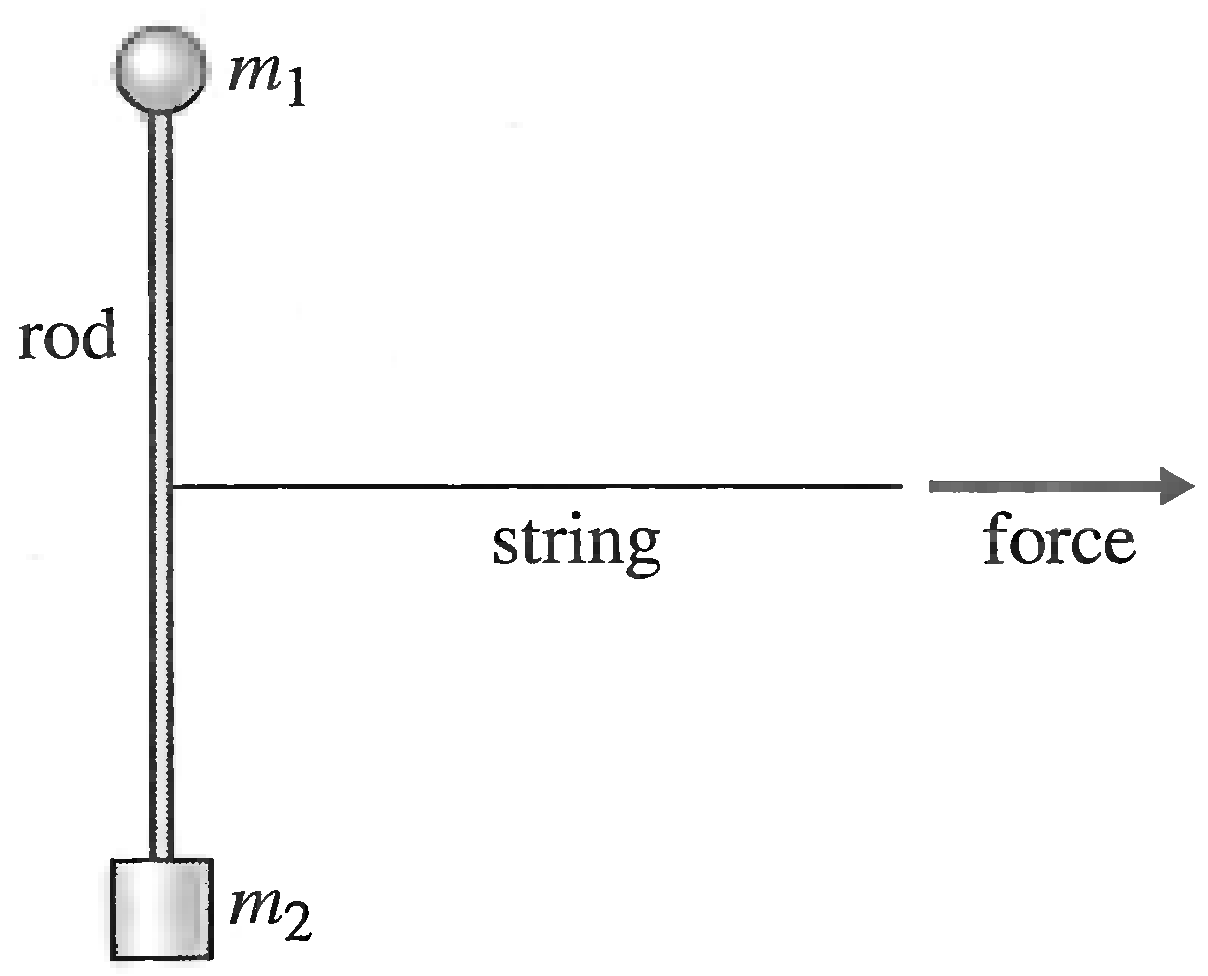
\includegraphics[width=0.5\columnwidth]{Fig2.2.png}
% \caption{เครื่องชั่งสมดุลความเฉื่อย (inertial balance) เปรียบเทียบมวล $m_1$ และมวล $m_2$ ของวัตถุสองชิ้นที่ติดอยู่ตรงปลายทั้งสองข้างของแท่งลวดแข็งเกร็ง มวลทั้งคู่จะเท่ากันก็ต่อเมื่อแรงที่ให้กระทำกับเส้นลวดตรงกึ่งกลาง จะทำให้มวลทั้งคู่เกิดการเร่งในอัตราที่เท่ากัน นั่นคือเส้นลวดนี้ต้องไม่มีการหมุนเกิดขึ้น}
% \label{Fig2.2}
% \end{figure}




% \subsection{แรง}
% \label{SubSec:Force}


% \section{กฎข้อหนึ่งและข้อสองของนิวตันในกรอบเฉื่อย}
% \label{Sec:FirstSecondNewtonLaws}



% \section{กฎข้อสามและการอนุรักษ์โมเมนตัม}
% \label{Sec:ThirdLawAndMomentumConservation}



% \section{กฎข้อสองของนิวตันในระบบพิกัดฉาก}
% \label{Sec:SecondNewtonLawInCarCoor}



% \section{ระบบพิกัดเชิงขั้วสองมิติ}
% \label{Sec:2DPolarCoor}


